\documentclass{report}
\usepackage{graphicx}
\usepackage{hyperref}
\author{Luke Maurits, \\
Add your name here, \\
If you contribute material, \\
Use alphabetical order}
\title{CLLARE Project Overview}
\begin{document}
\maketitle
\tableofcontents

\chapter{Introduction}

\section{What is CLLARE?}

The Collaborative Lunar Landing and Research (CLLARE) project is a proposed spaceflight project with the goal of landing a single human on the moon and returning them safely to Earth.  By using a reduced crew size, modern technology and a design philosophy emphasising simplicity and reusability, CLLARE endeavours to be an extremely low-cost project in comparison to Apollo or Constellation.

CLLARE is an ``open source'' spaceflight project.  What does this mean?  It means that documents such as this one and others which describe CLLARE in intimate technical detail, including spreadsheets and CAD files, are available for free under the Creative Commons Attribution Sharealike 3.0 license, so that anybody can copy, distribute and modify them.  It means that computer code to handle every aspect of planning and running CLLARE is available for free under the GNU General Public License 3,0, so that anybody can copy, distribute and modify it.  Anybody who has the desire, determination and money can build and launch the CLLARE hardware without any fear of legal issues (at least not from the people who planned CLLARE - some countries may have restrictions on who can launch what into space, when and where).  It means that anybody with the interest and knowledge can help refine the CLLARE project.

\section{Who is organizing CLLARE?}

CLLARE is a project of the Collaborative Space Travel and Research Team (CSTART).  CSTART is a non-government, non-profit space agency run by volunteers.  It provides online services to facilitate the planning and promotion of open source projects related to space travel and space research, like CLLARE.  It also attempts to raise the money required to fund these projects, or at least to fund the construction of proof--of--concept mock ups.  In the future CSTART may organize and fund space travel and research related prizes, with the condition that all entries are released under open source licenses at the end of the competition.

\section{How can I get involved in CLLARE?}

\section{How can I suggest changes/corrections/improvements to this document?}

%%%%%%%%%%%%%%%%%%%%%%%%%%%%%%%%%%%%%%%%%%%%%%%%%%

\chapter{Project Overview}

\section{Mission Overview}

The CLLARE mission is based around a Lunar Orbit Rendezvous (LOR) structure.  A spacecraft composed of several connected modules is launched into a low Earth ``parking orbit'', using a multiple stage rocket booster.  Following successful completion of various checks and tests, a Trans Lunar Injection (TLI) burn is performed, taking the spacecraft out of LEO and putting it on a lunar free return trajectory: a trajectory such that, with no further changes in velocity, the craft will travel close enough to the moon for the moon's gravitational field to cause reversal in its direction, putting it on a return course for Earth.

Once the spacecraft is sufficiently close to the moon, a lunar capture burn slows the spacecraft down to such a speed that it enters a low lunar orbit.

Once the lunar rendezvous has been completed, a lunar escape burn accelerates the spacecraft to a sufficiently high speed to escape the moon's gravitational field, leaving it on a course bound for Earth.

\section{Core CLLARE Hardware}

The CLLARE project is based around a set of modular hardware items, referred to as the core CLLARE hardware.  By combining items from the core hardware in appropriate configurations, a number of different mission types can be flown.  This approach allows a gradual progression toward the ultimate lunar goal.

The sections below introduce the core hardware items.  Figure \ref{fig:cm_configs} shows the various configurations of the hardware.  Chapter \ref{chap:detailed} describes more detailed descriptions of each hardware item and its subsystems, including diagrams.

\subsection{The CLLARE Command Module}

The \href{http://cstart.org/wiki/CLLARE_Command_Module}{CLLARE Command Module} (CM) is a one-person spacecraft in the ``truncated cone and cylindrical nose'' shape of the Mercury and Gemini spacecraft, which strongly influenced its design.  The CM contains sufficient onboard supplies of all required consumables to support its occupant for a duration of 24 hours, including support for one repressurisation of the capsule after extra vehicular activity (EVA) via an ingress-egress hatch.  An ablative heat shield permits the CM to reenter the Earth's atmosphere.  The CM will be capable of landing in water and possible also on land.  Suggested landing options include parachute, paraglider and ballute.  The CM will be designed to be as reusable as possible.

As a stand alone unit, the CM is capable of supporting only suborbital flights, making it functionally equivalent to early (suborbital) flights of the US Mercury craft.  More ambitius flights, including lunar landing missions, are facilitated by the use of a family of attachable modules.

\subsection{The CLLARE Retro Module}

The \href{http://cstart.org/wiki/CLLARE_Retro_Module}{CLLARE Retro Module} (RM) is a small, cylindrical module which attaches to the rear of the CLLARE CM.  The module contains a set of small and simple rockets (either solid or hybrid fuelled).  The module facilitates the use of the CM for orbital flights, by providing the means to deorbit such a CM.  The manner in which the RM attaches to the rear of the CM is such that the two modules can be separated after a deorbit burn, prior to reentry.  The RM is not equipped to survive reentry and burns up in Earth's atmosphere.

A CLLARE CM-RM combination is functionally equivalent to later (orbital) flights of Mercury or, if EVA is performed, early flights of the US Gemini craft.

\subsection{The CLLARE Mission Extension Module}

The \href{http://cstart.org/wiki/CLLARE_Mission_Extension_Module}{CLLARE Mission Extension Module} (MEM) is a cylindrical module which attaches to the rear of the the CM.  The module contains sufficient supplies of all required consumables to extend the CM's standalone endurance of 24 hours to a total of 7 days.  Consumables are conveyed from the MEM to the CM through an umbillical system which penetrates the CM's heat shield in a controlled manner.

The rear end of the MEM is sufficiently similar to the rear end of the CM that a CLLARE Retro Module can be attached to it, facilitating long-duration orbital missions.  In this configuration the MEM and RM are detached as a single unit prior to reentry.  The MEM is not equipped to survive reentry and burns up along with the RM.

A CLLARE CM-MEM-RM combination is functionally equivalent to the later flights of Gemini.

\subsection{The CLLARE Propulsion Module}

The \href{http://cstart.org/wiki/CLLARE_Propulsion_Module}{CLLARE Propulsion Module} (PM) is a cylindrical module which attaches to the rear of a CLLARE Command Module or Mission Extension Module.  The module contains a set of propellant tanks and contains a liquid bipropellant rocket at its end.  The PM is able to provide large changes in velocity to a CM or CM-MEM combination, allowing high-altitude Earth orbital flights or circumlunar flights.  The PM can also be used to perform deorbit burns, replacing the Retro Module for flights using a PM.  The PM is not equipped to survive reentry and burns up along with any other modules.

A CLLARE CM-MEM-PM combination is functionally equivalent to an Apollo Command Module and Service Module (CSM) combination (with no docked Lunar Module) - the MEM-PM combination is roughly functionally equivalent to the the Apollo SM.

In principle, multiple MEMs and PMs could be combined behind a single CM to allow arbitrarily long and distant flights, but launching such combinations would eventually become infesible.

\subsection{The CLLARE Lunar Mission Module}

The \href{http://cstart.org/wiki/CLLARE_Lunar_Mission_Module}{CLLARE Lunar Mission Module} (LMM) is a large cylindrical module which attaches to the rear of a CM-MEM combination.  The module provides all the facilities required to facilitate a lunar landing mission.  It includes a set of propellant tanks similar in design to those of the Propulsion Module, but larger (to support additional lunar capture and lunar escape burns) and space for the CLLARE Lunar Lander (see below) to dock.  Two ideas have been proposed for propulsion: in one, the LMM has a cluster of engines at its end, these engines being identical to thoseused on the PM; in the other, the Lunar Lander's engine (which is also identical to the PM engine) is used to provide propulsion.

A CLLARE CM-MEM-LMM combination is functionally equivalent to the full Apollo Spacecraft (i.e. Command Module, Service Module and Lunar Module).

\subsection{The CLLARE Lunar Lander}

The \href{http://cstart.org/wiki/CLLARE_Lunar_Lander}{CLLARE Lunar Lander} (LL) is a light weight, open cabin lunar landing craft.  Unlike the Apollo lunar lander (and like the planned Soviet lunar lander), the LL is not composed of two separable stages.  The entire structure undergoes a lunar descent and a lunar ascent, with the same engine and set of fuel tanks used for both directions.  The lunar lander's engine is a liquid bipropellant rocket and is the same engine as used for the CLLARE Propulsion Module and some versions of the Lunar Mission Module.

\begin{figure}[h] \label{fig:cm_configs}
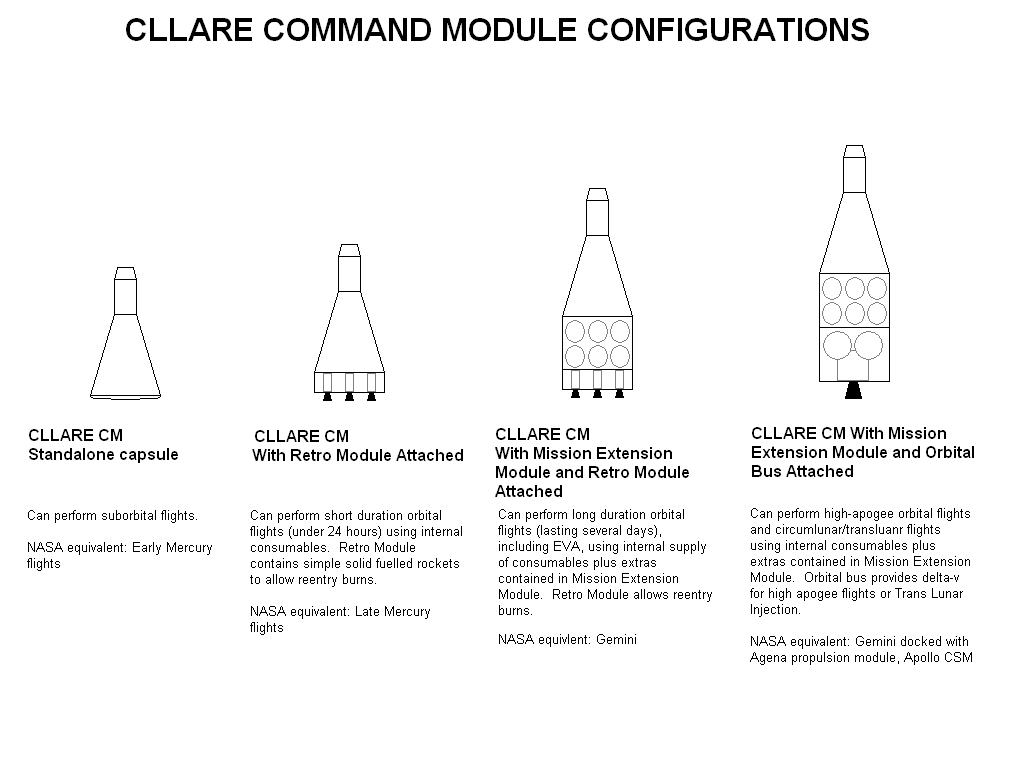
\includegraphics[angle=270, scale=0.6]{images/cllare_cm_configs}
\caption{Various configurations of the CLLARE core hardware (somewhat outdated).}
\end{figure}

\section{Launch Options}

\subsection{Suborbital missions}

\subsection{Circumlunar missions}

\subsection{Lunar landing missions}

The proposed lunar landing configurations (CM-MEM-LMM) have estimated total masses in the vicinity of 8000 kg (see Chapter \ref{chap:numeric} for details of these estimates).  The Falcon 9 booster is capable of lifting approximately 10,000 kg of payload into LEO.

\section{A proposed program of launches}

CLLARE 1: Unmanned suborbital flight (closely monitored crash test dummy in CM, full telemetry reporting)

CLLARE 2: Manned suborbital flight

CLLARE 3: Unmanned orbital flight (closely monitored crash test dummy in CM, full telemetry reporting)

CLLARE 4: Manned orbital flight, no EVA

CLLARE 5: Manned orbital flight, including EVA

CLLARE 6: Unmanned high altitude orbital flight

CLLARE 7: Manned high altitude orbital flight

CLLARE 8: Unmanned circumlunar flight

CLLARE 9: Manned circumlunar flight

CLLARE 10: Manned lunar landing flight

%%%%%%%%%%%%%%%%%%%%%%%%%%%%%%%%%%%%%%%%%%%%%%%%%%

\chapter{Numerical Analysis} \label{chap:numeric}

In this chapter we present estimates, principled arguments and calculations to estimate the total mass and cost of flying various configurations of the CLLARE core hardware.  We conclude that a complete lunar landing mission based on the CLLARE hardware should cost no more than US\$50,000,000.

\section{Astrodynamics}

Delta-vs and a rough timeline go here.

\section{Mass figures}

\subsection{Empty structure masses}

\subsection{Consumables masses}

\subsection{Fuel masses}

In this section we use the Tsiolkovsky rocket equation to estimate the required fuel masses for the mission, considering various fuel options.

(Get figures for LOX/H2, LOX/CH4 LOX/RP-1)

\subsection{Total launch masses}

The table below summarises estimated total launch masses for various configurations of the CLLARE core hardware.

\begin{tabular}{ | l | c | }
\hline
Configuration & Estimated total mass (kg) \\
\hline
\hline
Suborbital (CM) & 1500 \\
\hline
Short Orbital (CM-RM) & 1600 \\
\hline
Long Orbital (CM-MEM-RM) & ??? \\
\hline
High Altitude Orbital, Circumlunar & ??? \\
(CM-MEM-PM) & \\
\hline
Lunar Landing (CM-MEM-LMM) & 8000 \\
\hline
\end{tabular}

\section{Cost figures}

\subsection{Fuel costs}

\subsection{Launch costs}

%%%%%%%%%%%%%%%%%%%%%%%%%%%%%%%%%%%%%%%%%%%%%%%%%%

\chapter{Detailed Hardware Descriptions} \label{chap:detailed}

In this chapter we present detailed descriptions of some of the CLLARE core hardware items.  Complete technical descriptions and diagrams of all hardware items will be compiled into a separate publication at a future time.

\section{The CLLARE Command Module}

\subsection{Structure and construction}

Discuss CM structure here.

\subsection{Reaction Control System}

The \href{http://cstart.org/wiki/CLLARE_CM_Reaction_Control_System}{CM's Reaction Control System} (RCS) provides pitch, yaw and roll control for the CM, to be used both during spaceflight and reentry. It is the CM's only self-contained means of propulsion.

\subsection{Power system}

The \href{http://cstart.org/wiki/CLLARE_CM_Power_System}{CM's power system} provides 12V and 24V DC power to other subsystems, generated by an array of atmosphere breathing methanol-water fuel cells with backup batteries.

\subsection{Environmental Control System}

The \href{http://cstart.org/wiki/CLLARE_Environmental_Control_System}{CM's Enviromental Control System} is responsible for maintaining a habitable environment inside the CLLARE Command Module cabin. This involves maintaining an appropriate oxygen level, pressure level, temperature and more.

\subsection{Communication System}

The \href{http://cstart.org/wiki/CLLARE_CM_Communication_System}{CM's Communication System} provides a number of communication services, including a bidirectional voice link between the CM and the ground, multiple one directional video links from the CM to the ground, a one directional telemetry link between the CM and the ground, and a one directional authenticated control link from the ground to the CM.

\subsection{Navigation System}

The \href{http://cstart.org/wiki/CLLARE_CM_Navigation_System}{CM's Navigation System} uses various hardware sensors and interactions with other subsystems to provide high accuracy estimates of position, orientation and velocity at all stages of the mission.  Plans for the navigation system include the use of an inertial measurement unit, radio round--trip--time and Doppler shift measuremets, StarTrackers and more.

\subsection{Computer System}

The \href{http://cstart.org/wiki/CLLARE_Main_Computer_System}{CM's Main Computer System} provides computational support for most other subsystems.

\section{The CLLARE Retro Module}

Discuss rocket options here.

\section{The CLLARE Mission Extension Module}

Discuss required consumables and storage options here: oxygen, nitrogen, methanol, water, anything else?

\section{The CLLARE Propulsion Module}

Discuss fuel options here.

Discuss cooling options here.

\section{The CLLARE Lunar Mission Module}

\section{The CLLARE Lunar Lander}

\subsection{Reaction Control System}
\subsection{Power system}
\subsection{Communication System}
\subsection{Navigation System}

\end{document}
